% Diagram for the "Programs move between languages" slide.
% Styled to match ../openxla-stack.tex: rounded boxes, Stealth arrows, blue for
% the parts that are ours, grey for the shared core. The StableHLO program is
% what {anvl} emits for function(x, y) x + y on two f32[3] arrays.
% Build: pdflatex programs-move.tex && pdf2svg programs-move.pdf programs-move.svg
\documentclass[tikz, border=8pt]{standalone}
\usepackage[T1]{fontenc}
\usetikzlibrary{arrows.meta, positioning, fit, backgrounds}

\newsavebox{\prog}
\begin{lrbox}{\prog}
\begin{minipage}{6.1cm}
\scriptsize
\begin{verbatim}
func.func @main(%0: tensor<3xf32>,
                %1: tensor<3xf32>)
    -> tensor<3xf32> {
  %2 = stablehlo.add %0, %1 : tensor<3xf32>
  return %2 : tensor<3xf32>
}
\end{verbatim}
\end{minipage}
\end{lrbox}

\begin{document}
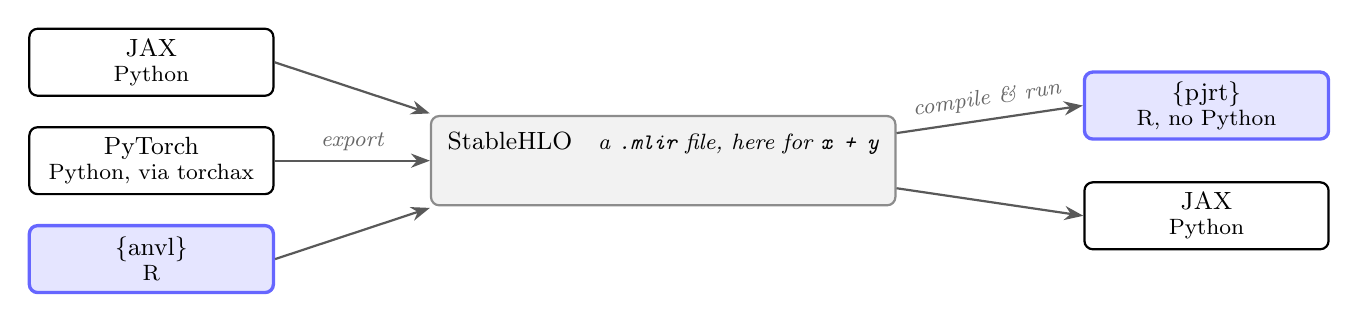
\begin{tikzpicture}[
  every node/.style={font=\small},
  box/.style={
    draw, rounded corners=3pt, thick,
    minimum width=3.1cm, minimum height=0.85cm, align=center
  },
  ours/.style={box, fill=blue!10, draw=blue!60, very thick},
  core/.style={box, fill=black!5, draw=black!45, inner sep=6pt},
  arr/.style={-{Stealth[length=2.4mm, width=1.8mm]}, thick, draw=black!65},
  lbl/.style={font=\footnotesize\itshape, text=black!60}
]
  % --- frontends -----------------------------------------------------------
  \node[box]  (jax)   at (0,  1.25) {JAX\\[-2pt]{\footnotesize Python}};
  \node[box]  (torch) at (0,  0)    {PyTorch\\[-2pt]{\footnotesize Python, via torchax}};
  \node[ours] (anvl)  at (0, -1.25) {\{anvl\}\\[-2pt]{\footnotesize R}};

  % --- the shared format, with an example program ---------------------------
  \node[core] (shlo) at (6.5, 0) {%
    StableHLO\quad{\footnotesize\itshape a \texttt{.mlir} file, here for \texttt{x + y}}\\[3pt]
    \usebox{\prog}};

  % --- where it runs --------------------------------------------------------
  \node[ours] (pjrt)  at (13.4,  0.7) {\{pjrt\}\\[-2pt]{\footnotesize R, no Python}};
  \node[box]  (jaxrt) at (13.4, -0.7) {JAX\\[-2pt]{\footnotesize Python}};

  \draw[arr] (jax.east)   -- (shlo.west |- 0, 0.6);
  \draw[arr] (torch.east) -- node[lbl, above] {export} (shlo.west);
  \draw[arr] (anvl.east)  -- (shlo.west |- 0, -0.6);
  \draw[arr] (shlo.east |- 0, 0.35)  -- node[lbl, above, sloped] {compile \& run} (pjrt.west);
  \draw[arr] (shlo.east |- 0, -0.35) -- (jaxrt.west);
\end{tikzpicture}
\end{document}
